 \begin{figure}[htb]	
 
   \centering
  \begin{tabular}{  c c c c  c}
    %\centering
    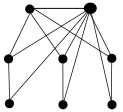
\includegraphics[width=2.5cm]{img/f1.png} 
    & 
    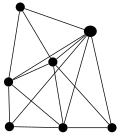
\includegraphics[width=2.3cm]{img/f2.png} 
    & 
    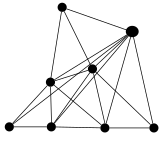
\includegraphics[width=3cm]{img/f3.png} 
    & 
    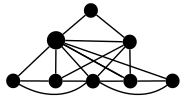
\includegraphics[width=3cm]{img/f4.png} 
    & 
    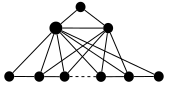
\includegraphics[width=3cm]{img/f5.png} 
    \\
    \footnotesize 
    (a)  \footnotesize Graph $F_1$. 
    & 
    \footnotesize (b) Graph $F_2$.
    & 
    \footnotesize (c) Graph $F_3$.
    & 
    \footnotesize (d) Graph $F_4$.
    & 
    \footnotesize (e) Graph $F_5(n),n\geq7$.
    \\%%Segunda linha
        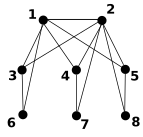
\includegraphics[width=2.5cm]{img/f6.png} 
    & 
    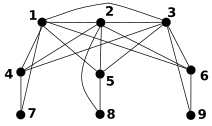
\includegraphics[width=3.5cm]{img/f7.png} 
    & 
    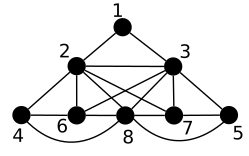
\includegraphics[width=3cm]{img/f8.png} 
    & 
    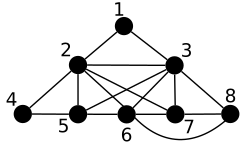
\includegraphics[width=3cm]{img/f9.png} 
    & 
    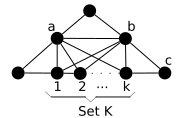
\includegraphics[width=3cm]{img/f10n.png} 
    \\ %%Segundo Bloco legendas
    \footnotesize 
    (f)  \footnotesize Graph $F_6$. 
    & 
    \footnotesize (g) Graph $F_7$.
    & 
    \footnotesize (h) Graph $F_8$.
    & 
    \footnotesize (i) Graph $F_9$.
    & 
    \footnotesize (j) Graph $F_{10}(n), n\geq  8$.
    %%Terceira linha de imagens
    \\%%Terceira linha
        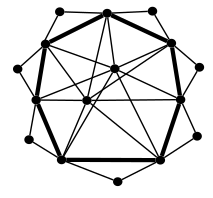
\includegraphics[width=3cm]{img/f11.png} 
    & 
    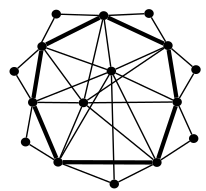
\includegraphics[width=3cm]{img/f12.png} 
    & 
    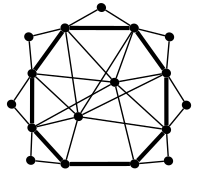
\includegraphics[width=3cm]{img/f13.png} 
    & 
    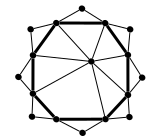
\includegraphics[width=3cm]{img/f14.png} 
    & 
    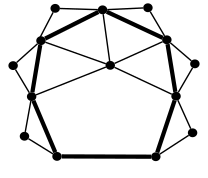
\includegraphics[width=3cm]{img/f15.png} 
    \\ %%Terceiro Bloco legendas
    \footnotesize 
    (k)  \footnotesize  $F_{11}(4k),k\geq2$. 
    & 
    \footnotesize (l)  $F_{12}(4k),k\geq2$.
    & 
    \footnotesize (m)  $F_{13}(4k+1),k\geq2$.
    & 
    \footnotesize (n)  $F_{14}(4k+1),k\geq2$.
    & 
    \footnotesize (o)  $F_{15}(4k+2),k\geq2$.
    
    \\ %Ultima linha Figuras
    
    && 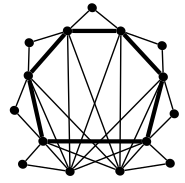
\includegraphics[width=3cm]{img/f16.png} &&
    
    \\%Ultima linha Legendas
    
    && \footnotesize (p)  $F_{16}(4k+3),k\geq2$. &&
    
    %\multicolumn{3}{c}{ \footnotesize (c) Another partial single bend representation of $H$ } \\
  \end{tabular}
 \caption{The 16 Chordal induced subgraphs forbidden to VPT (the vertices in the cycle marked by bold edges form a clique).}
 %, see  more in~\cite{leveque2009characterizing,tondato2009grafos}
 \label{fig:16proibidos}
\end{figure}  
 